\documentclass[11pt]{report}
\setlength\parindent{24pt}
\usepackage[utf8]{inputenc}
\usepackage{indentfirst}
\usepackage{enumitem}
\usepackage{quoting}
\usepackage{float}
\usepackage{graphicx}
\usepackage[export]{adjustbox}
%--------- Chapter & title spacing ----------------------------
\usepackage{titlesec}
\titleformat{\chapter}[display]
{\normalfont\huge\bfseries}{\chaptertitlename\ \thechapter}{20pt}{\Huge}
% this alters "before" spacing (the second length argument) to 0
\titlespacing*{\chapter}{0pt}{-40pt}{0pt}
%------- Quotation spacing ------------------------------
\quotingsetup{vskip=0pt}
%------ [sub*]sections spacing ---------------------------
\usepackage{titlesec}
\titlespacing\section{0pt}{12pt plus 4pt minus 2pt}{0pt plus 2pt minus 2pt}
\titlespacing\subsection{0pt}{12pt plus 4pt minus 2pt}{0pt plus 2pt minus 2pt}
\titlespacing\subsubsection{0pt}{12pt plus 4pt minus 2pt}{0pt plus 2pt minus 2pt}
\addtolength{\topmargin}{-3cm}
\addtolength{\textheight}{3cm}
%-------- Pseudo code --------------------------------
\usepackage[ruled,vlined]{algorithm2e}
\iffalse ----------------Title / Author / Date ------------------- \fi
\title{\textbf{Internship report: \\
			LIS\\  Minimal Manhattan network}}
\author{ABDEL WAHAB Ismail}
\date{25 April 2020}

\iffalse ------------------ First Page --------------------------- \fi    
\usepackage{amssymb}
\begin{document}
\maketitle
\thispagestyle{empty}
\renewcommand{\contentsname}{Summary}
\tableofcontents
\newpage

\iffalse --------------  Document Content-------------------------- \fi

\part{LIS and intership's subject}
\chapter{Presentation of the Laboratory}
\section{Creation of the structure}
The Computer Science and Systems Laboratory (LIS) in french "Laboratoire d’Informatique et Systèmes", is a structure that is the resulting of the merge of two laboratories. It is from The "Laboratoire Fondamentale de Marseille" (LIF) and also from the "Laboratoire des Sciences de l'Information et des Systèmes (LSIS) that the LIS was created.

\section{Supervisors and partner of the LIS}
LIS is a research lab which is put under the supervision of the "Centre National de la Recherche Scientfique" (CNRS), Aix-Marseille University and University of Toulon. The LIS also has as a partener the "Ecole Centrale de Marseille" (ECM).

\section{Localisation of the laboratory}
The Computer Science and Systems Laboratory is located in France and is split upon two cities, Marseille and Toulon. On Marseille we can find two places that are used by the LIS: the first one being on the university campus of Saint-Jérôme and the other on Luminy. You can also find the LIS in Toulon on the campus of the University of Toulon.
 
\section{Workforce}
Spread over all of theses locations, the LIS is represented by 375 members from which we can count:
\begin{itemize}[noitemsep, nolistsep]
	\item{190 tenure researchers and professors}
	\item{125 doctoral students}
	\item{40 post-docs }
	\item{20 technical staff}
\end{itemize} 

\section{Reason behind the creation of the LIS}
The Computer Science and Systems Laboratory was created so that we can use the strengths and competences of both LSIS and LIF together in order to meet and overcome new scientific challenges.

\section{Hierarchy of the laboratory}
While keeping this objective in head this laboratory created four departments. Each of them will inherit and focus their research on a specific domain that was previously studied by the LSIS, the LIF or both of them.
Those four departments are:
\begin{itemize}[noitemsep, nolistsep]
	\item{Calculus}
	\item{Data science}
	\item{Signal and image}
	\item{System Analysis and Automatic Control}
\end{itemize}
Also each department is divided into subgroups working on specific topic treated by their department.

\subsection{Calculus department}
This department of the LIS was created with the objective to focus on some specific research activities like: Theoretical computer science, logic, obviously algorithmic and complexity, geometric and topology, but also quantum computing and artificial intelligence.
\subsection{Data science department}
Nowadays we know the importance of data, should it be founding it, treating data or even analyzing it. So at the LIS a department is dedicated to the science of data, they are working on  machine learning which is a growing technology, natural language processing that is also an upcoming technology that will be vastly used, data mining and information retrieval to collect data which is as important as computing it, and of course artificial intelligence that work hand in hand with machine learning.
\subsection{Signal and image department}
The art of manipulating visual data is represented by this department. They especially work on  image processing to treat images an recover data from them. But also on audio and bio-signal processing, medical imaging and here we see the importance of this department along the fact that they work with the medical field. And lastly image modeling is a topic that this department is competent to treat.
\subsection{System Analysis and Automatic Control (ACS) department}
The last department to be presented is making research on control theory, diagnostic, decision theory, system simulation and modeling too. This department is focus on the analysis of systems, their correctness and also the automatic controls that can be made over them. % done ??? can be larger !
\chapter{Subject matter}
\section{Introduction to subject matter}%%%%%%%%%%%%%%%%%%%%%%%%%%%%%%%%%
In this internship we will try to understand the properties of a minimal Manhattan network and try to find it upon some given data.

\noindent For that we need to firstly describe what is a Manhattan network.
\subsection{Manhattan network}
A Manhattan network is defined over a set of points in a x dimensional space. With x that can go from 2 to +$\infty$ (Manhattan network on a 1 dimensional space is trivial: is just a line going through all points). Of course the more dimensions are defining your space, the harder is the problem.\newline


\noindent To create a Manhattan network the rules are simple:
\begin{enumerate}[noitemsep, nolistsep]
	\item{Define the space we are working in (number of dimensions)}
	\item{Define the unit ball of this space}
	\item{Give a cloud of points(terminals) on this space}
	\item{If needed use \emph{unit coordinates} to simplify computations}
	\item{Connect every possible pairs of points with edges using only two directions allowed by the unit ball}
\end{enumerate}
	In this report we will guide you to understand all words and steps described in these instrucitons. 
	
	To have an quick description of a Manhattan network you just need to know that, over a given set of points in a x dimensional space, we will have to connect every possible pairs of points with edges. Those edges can only be in two directions. 
	
	For example in the normed plane the edges are either vertical either horizontal, you can see an example just below in Fig.2.1 . 
	
\begin{figure}[H]
  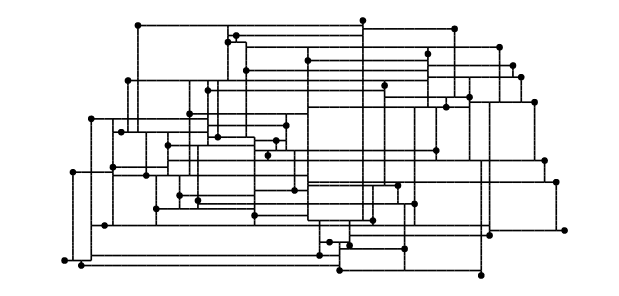
\includegraphics[width=\linewidth]{img/mn_example.png}
  \caption{A minimal Manhattan network.}
  \label{fig:mn_expamle}
\end{figure}
But in general any two directions can define the edge's possible layouts for our network.
\subsection{Minimal Manhattan networks}
A Minimal Manhattan network has obviously the same properties as a Manhattan network, but we add to them a constraint: the sum of the length of all edges (lines in the network) must be the lowest possible.

It is by using numerous algorithms and data structures that we will ensure that what we create is a real minimal Manhattan network.

This simple constraint will totally change the way we approach the problem and how we shall solve it. By trying to find  a minimal solution we are greatly increasing the complexity of the work that will be needed to do to answer our question.

\section{Creation of the first paper}%%%%%%%%%%%%%%%%%%%%%%%%%%%%%%%%%%%%%%%%%
Gudmundsson, Levcopoulos and Narasimhan are three scientists that worked together in the 90's on this specific topic. Finding a Minimal Manhattan network for a given set of terminals as quick as possible was their objective. In fact at the time it wasn't known that this problem was actually NP-Hard, and required a lot of calculation to be solved.

This is why after a long work the pioneers of the MMN published two algorithms with factors 4 and 8. Knowing that this problem was bind to be difficult they emitted the conjecture that a factor 2 algorithm must exist.

And it is at this time that they opened the door to a vast community of researchers to work on the topic and also variants of this problem.

But before going deeper into the explanation we need to define the elements that we are going to work on. 

\section{Origins of the topic}%%%%%%%%%%%%%%%%%%%%%%%%%%%%%%%%%%%%%%%%%%%%%%%
The minimal Manhattan network problem was in fact formulated in 1999 by Gudmundsson, Levcopoulos and Narasimhan whom found the two approximating algorithms. 

Moreover they conjectured the existence of an approximating algorithm of factor 2, without having any idea if they were close to find this algorithm or not. Nevertheless that this conjectured algorithm could give the solution to our problem with a cost lower than two times the optimal cost to find the optimal solution.

Actually, this algorithm was found in 2005 by my internship's mentors, Y.Vaxes and V.Chepoi, along with K.Nouioua and N.Catusse by using rounding method on a factional optimal solution, and then coupling it with a primal-dual algorithm.

Later other variants of this problem were studied, like for example the generalization of the problem to the normed plane with polygonal balls (in the l1-metric this polygon ball is a lozenge and not a always a square). And for this version of the MMN an algorithm factor 2.5 was found [2].

\part{Calculate a minimal Manhattan network}
\chapter{Terminals}
\section{Points in the space}
Points in the space are named \textbf{terminals}, in this paper a terminal will refer to a point in the space.\newline

For our study, we will focus ourselves on two dimensional space, but keep in mind that with a little more work and a lot of adjustments, all of what you are going to discover can be applied to more dimensions.

A point will be defined with Cartesian coordinates. In this paper we will note terminals with lower case letters. We will talk of a point \textbf{\emph{p}} or a point \textbf{\emph{q}} for example.

When speaking about one of the coordinate of a point we will use subscript notation as: $x_p$ for the x coordinate of the point \emph{p}.
\section{A set of terminals to begin with}%%%%%%%%%%%%%%%%%%%%%%%%%%%%%
To work on finding a MMN, we have to understand on what data we are searching this network. The objective of such a network is to \textbf{connect each an every possible pairs of points} in a set of terminals (in our case on the plane).

In fact connecting all possible pairs of terminals given a list of terminals is not difficult at all (for example just create the complete grid of your set of terminals: 

\begin{algorithm}[H]
\SetAlgoLined
 \caption{Complete grid from a set of Terminals "T"}
\KwResult{The complete grid of a set of terminals in 2D }
 lowX = lowest x value of all terminals\;
 highX = highest x value of all terminals\;
 lowY = lowest y value of all terminals\;
 highY = highest y value of all terminals\;
 completeGrid = [ An empty list of lines ]\;
 \For{Every terminal t in our set of terminals}{
 Add to completeGrid the line from (lowX,$y_t$) to (highX,$y_t$)\;
 Add to completeGrid the line from ($x_t$,lowY) to ($x_t$,highY)\;
 }
 return completeGrid\;
\end{algorithm}

Here we can see that collecting the minimal and maximal x and y coordinates, is a linear operation and the creation of both lines are also linear operations. In conclusion a naive Manhattan network can be found in O(n). 

However, generally this naive answer to our problem is far from the minimal Manhattan network. And here is the trick, this is what we want a \textbf{\emph{Minimal}} Manhattan network.

\section{Terminal's properties}
Before going further in the subject, we will need to define some properties of our terminals.

These properties are the core of our computation as we will use them in order to run some algorithms over the set of terminals. As it is of high importance, the definition of these properties are given here. 
\subsection{Domination} %%%%%%%%%%%%%%
Let T bet a cloud of points in two dimensions.

Let \emph{p} and \emph{q} be two terminals of T.

\noindent It is said that \emph{p} dominates \emph{q} \underline{if and only if}:
\begin{enumerate}[noitemsep, nolistsep]
	\item{$\forall t \in T : d(p,t) \leq d(q,t)$}
	\item{$\exists t' \in T : d(p,t) < d(q,t)$}
\end{enumerate} 
With d(p,t) the distance between \emph{p} and \emph{t}, that is calculated based on the metric that we use. The next whole chapter is dedicated to, and will explain, metrics and how do we calculated distances.

In this definition we need to note that no point can be dominated. As for all \emph{t} in T d(p,t) must be lower or equal to d(q,t), (of course we take in consideration that \emph{p} and \emph{q} are different points) then \emph{t} could be \emph{q}. In this case then it is impossible to have $d(p,q)\leq d(q,q)$.

In any case if a terminal \emph{p} dominates another terminal \emph{q} we denote this property by: $ p \succ q $
\subsection{Efficiency}%%%%%%%%%%%%%%%%
A point \emph{p} is said to be efficient if $\neg\exists q$ and \emph{q} dominates \emph{p}. In other words: a terminal is said efficient if no other terminal is dominating it.

As no points should be dominated, in fact all terminals in our cloud of points are efficient terminals.
\subsection{Equivalence} %%%%%%%%%%%%%%
Let A be a subset of  our space $R^m$ : $A \subset R^m$.

Let \emph{p} and \emph{q} be two points of T: $p \in T$ and $q \in T$

\noindent Our two points, \emph{p} and \emph{q} are said to be equivalent by A \underline{if and only if}:
\begin{itemize}[noitemsep, nolistsep]
	\item{$\forall a \in A : d(p,a) = d(q,a)$}
\end{itemize} 

So as we see here, for a part of our space we can define two points as equivalent if and only if for all terminals in this part, our two points are equidistant to each and every point in this part.

We denote this property as: $p \simeq_{A} q$ if p and q are equivalent by A.
\chapter{Metrics}
\section{Definition}%%%%%%%%%%%%%%%%%%%%%%%%%%%%%%%%%%%%%%%%%%%%%%%%%%%%%
A metric is a function, more precisely a distance function. It is used to define how do we calculate the distance between two elements in a set.

This function takes as input two elements from a set and outputs the distance between them. Of course their are many ways to calculate a distance between two elements based on what you want and what type of data you are working on.

For a classic presentation we will introduce the l2-metric. Later in this report we will use the l1-metric as it is the one that is important for us.
\section{Example of metrics}%%%%%%%%%%%%%%%%%%%%%%%%%%%%%%%%%%%%%%%%%%%%%%%%
\subsection{The l2-metric}%%%%%%%%%
For the sake of simplification we will just present you the l2-metric, which is the one that we use in the "all days" world.

In fact, the \textbf{l2-metric} is also know as the \textbf{Euclidean distance} and uses the formula relative to the Pythagorean theorem:
	\[d_2(p,q)= d_2(q,p) = ||p - q|| = \sqrt{(x_q-x_p)^2+(y_q-y_p)^2}\]
	
This is the casual way to calculate distances on a map or between points.
\subsection{The l1-metric}%%%%%%%%%%
	And now as simple as it is, the \textbf{l1-metric} is just another way to calculate the distance between two points p and q:
	\[ d_{1}(p,q)= d_{1}(q,p) = |x_p-x_q|+|y_p-y_q|\]
What is interesting in this metric here, is that we calculate a distance based of the variation of x coordinates and the variation of y coordinates.

Which means that we give some importance to the fact that we can only create edges on those two axes. This will be really useful later when we will speak about Pareto envelopes and minimal Manhattan network in more details.
\chapter{Interval with triangular equality}
Before jumping in and defining what is the Pareto envelope of our set of terminals, or even saying why will we calculated it, we need to define the interval of points that respect the triangular equality.

\section{Triangular inequality/equality} %%%%%%%%%%%%%%%%%%%%%%%%%%%%%%%%%%%
\noindent The Triangula \textbf{in}equality states that:
\begin{quoting} \begin{verbatim}
  For a triangle the sum of the length of any two sides
of this triangle, must be greater than the length of the third side.
\end{verbatim} \end{quoting}
Which means that: let $abc$ be a triangle:
\begin{itemize}[noitemsep, nolistsep]
	\item{$d(a,b)+d(b,c) > d(a,c)$}
	\item{$d(a,c)+d(c,b) > d(a,b)$}
	\item{$d(b,a)+d(a,c) > d(b,c)$}
	\newline
\end{itemize}

	Now take in consideration two point \emph{a} and \emph{b}, all \emph{c} points that respect the triangular equality are the ones that do not verify the triangular inequality which means that:
\begin{itemize}[noitemsep, nolistsep]
	\item{$d(a,c)+d(c,b) \leq d(a,b)$}
	\newline
\end{itemize}

\section{Interval and metrics} %%%%%%%%%%%%%%%%%%%%%%%%%%%%%%%%%%%
	But as we defined previously d(x,y), we know that this notation depends on the metric that we use. Moreover, depending on which metric we use the set of points that will respect the triangular equality will differ. Here are some examples of this set depending on the metric used:
\begin{figure}[H]
  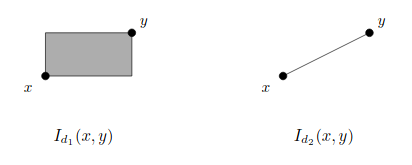
\includegraphics[width=\linewidth]{img/interval_example.png}
  \caption{Triangular equality interval depending on the metric.}
  \label{fig:interval_example}
\end{figure}

As you can see on the right, this set is just all the points on a straight line between \emph{x} and \emph{y}. In fact as we use the l2-metric (Cartesian distance) we fall back on our feet with the casual definition of the triangular inequality.

Nevertheless, on the left we see that for the l1-metric this interval is a square, with the segment [\emph{x},\emph{y}] being a diagonal of this square. And you can see that after doing the calculation we actually end up with this shape for all points that respect the triangular equality.

\section{Usage of intervals} %%%%%%%%%%%%%%%%%%%%%%%%%%%%%%%%%
Also as we will work a bit with the l1-metric, this result will be really useful for future computations.\newline

All the points that respect the triangular equality can be regrouped in a set. This set will simply be called interval between x and y for the metric $d_1$(resp. $d_{metric\_identifier}$).

It is base on this interval that we will also define the Pareto envelope of our set of terminals.

Note: As the construction of the Pareto envelope can be linked to the interval between all pair of points, and as this said interval depends on the metric that we use to calculate distances, \textbf{the Pareto envelope of a set of terminals depends on the metric that we use}.

\section{Used notation}
By defining this interval we now can have a way to start and work our way to the Pareto envelope of our set. 

This interval will be noted as: $I_{d}$.

\noindent With $d$ the identifier of the metric used to calculate this interval.
\chapter{Unit coordinates}
\section{What are unit coordinates}%%%%%%%%%%%%%%%%%%%%%%%%%%%%%%%%%
	Granted that we are working in a two dimensional space, all coordinates are more likely to be real numbers than natural numbers.
	Moreover our system would be useless if we were only working on discrete coordinates, where our world and the way we measure distance is not discrete.
	
	However we can counter this by having a tool or an algorithm that can convert two dimensional coordinates into discrete coordinates. Unit coordinates are a way to locate points in space with only round numbers.
	
	Additionally this will restrict the space we are working on from $\mathbb{R}^2$ to a grid containing all of our terminals.
	
	This tool would greatly lower our computation time and will make our future algorithm more easier to implement.
\section{Why do we use them}%%%%%%%%%%%%%%%%%%%%%%%%%%%%%%%%%%%%%%
	Under those circumstances, as said it make implementation of future algorithm simpler as we are standardizing the way we are talking about coordinates and points. As a result all future algorithm will share the same references to coordinates and it will be simpler to consecutively run algorithms on the same data.
	
	Furthermore speaking of data, this will also define the data structure used to store our terminals. In my own implementation terminals in $\mathbb{R}^2$ are read from a CSV file and stored as a list. Just after that I use an algorithm designed by myself to convert those real coordinates into unit coordinate.

\section{Recovering original coordinates after computations}%%%%%%%%%%
Despite having unit coordinates making our job easier, we need at the end of all our computation to be able to transition back to the real points in $\mathbb{R}^2$ because otherwise using unit coordinates would not make sens.

For this we created a specific data structure (in my implementation a python dictionary) to link each real point to his unit coordinate translation by our algorithm.\newline

After having found a minimal Manhattan network for our set of unit coordinates points, we will use the fact that in the view of Pareto envelope and Manhattan network (and it has to work for both as the first is used to create the second), unit coordinate is an \textbf{isotone mapping} of our points.

Meaning that for a partial order relation \emph{\textbf{R}}, applying an isotone mapping \textbf{will not} change the order of any elements in \emph{\textbf{R}}.

And as a matter of fact we have to remember ourselves that terminal domination is a partial order relation that is used to define all of the structure we are talking about.

If we keep this relation untouched, we just shown that if we found a MMN for our unit coordinate grid, it is the same thing than finding a MMN for the set for terminals in $\mathbb{R}^2$. We will just have to convert our point back to what they were in $\mathbb{R}^2$. %TODO ALGO to convert to unit coords
\chapter{Pareto envelopes}
\chapter{Minimal Manhattan network (MMN)}
At this stage, most of the work is already done, we just only miss the computation of the minimal Manhattan network.

Clearly, with all the data we have now from our set it will be (with the usage of some tricks) not that hard to compute it.

Now that we have the Pareto envelope of our set, we just need to find a generating set over our terminals and satisfy it.

In this chapter we will cover what is a generating set and why satisfying such a set is equivalent to finding a minimal Manhattan network.
\section{Generating set}%%%%%%%%%%%%%%%%%%%%%%%%%%%%%%%%%%%%%%%%
\noindent Let A be a generating set over a cloud of terminals T.

\noindent A respects the following assertions:
\begin{enumerate}[noitemsep, nolistsep]
	\item{A is a subset of T: $A \subseteq T$ }
	\item{Connecting all pairs of A \textbf{implies} All pairs of T are connected }
\end{enumerate}

\noindent As a matter of fact, we now know that we can in order to find a minimal Manhattan network, try to find a generating set over our terminals.

By studying two specific geometrical shapes in our set T we will be able to create such a generating set, thus solving our problem: finding a minimal Manhattan network.
\section{Terminal's neighbours}%%%%%%%%%%%%%%%%%%%%%%%%%%%%%%%%%
As we are trying to find geometric shapes that can be defined as a generating set, we need to be able to talk about the neighbours of a point.

In fact we will create appropriated data structures so that we keep in memory the neighbours of each point.

\subsection{$Q_i$, $A_i$, and $O_i$ dictionaries.}
\noindent For that we will use dictionaries:
\begin{itemize}[noitemsep, nolistsep]
	\item{Step one: As you can see in \emph{Fig 8.1} is for a point to divide the space around it in four squares. ($Q_i$ $|$ $\forall i \in [1,4]$) }
	\item{Step two: For each $Q_i$ we will create the appropriated $A_i$ and $O_i$}
\end{itemize}

\begin{figure}[H]
  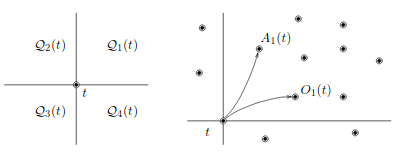
\includegraphics[width=\linewidth]{img/terminal_neighbours.png}
  \caption{Terminal's neighbours}
  \label{fig:terminal_neighbours}
\end{figure}

\subsection{Definition of $A_i$ and $O_i$}
\noindent Let \emph{p} and \emph{q} be two point in T. ($p \in T$ and $q \in T$)

\noindent Let $A_i$ be linked to $Q_i$. (i.e $A_1$ is linked to $Q_1$ for example)

\noindent Let $A_i$ be a dictionary from a point to another (i.e $A_i(point1) = point2$)\newline

\noindent $A_i(p) = q$ means that:
\begin{itemize}[noitemsep, nolistsep]
	\item{ $q \in Q_i$}
	\item{ \emph{q} is the closest point to the a \textbf{vertical line} going through \emph{p}}
\end{itemize}

\noindent $O_i(p) = q$ means that:
\begin{itemize}[noitemsep, nolistsep]
	\item{ $q \in Q_i$}
	\item{ \emph{q} is the closest point to the an \textbf{horizontal line} going through \emph{p}}
\end{itemize}

\subsection{Algorithm to create $A_i$ and $O_i$}
In this part I will present you an algorithm to generate $O_1$.

\noindent \textbf{Note:} All other dictionaries can be created similarly just by giving small modifications on the following algorithm.
 
\begin{algorithm}[H]
\SetAlgoLined
 \caption{Calculate $O_1$}
\KwResult{The $0_1$ dictionary properly filled }
Sort T  by increasing ordinates and increasing abscissa\;
$O_1 = $ An empty dictionary\;
toTreat = An empty stack\;
$toTreat.push( t_0)$\;
\For{ i=1 to n }{
	\While{ First element of toTreat has an abscissa $\leq x_{t_i}$ }{
		s = toTreat.pop()\;
		$O_1(s) = t_i$\;
	}
	toTreat.push($t_i$)\;
}
\While{The stack toTreat is not empty}{
	s = toTreat.pop()\;
	$O_1(s) = \o$\;
}
return $O_1$
\end{algorithm}


\section{Strips}%%%%%%%%%%%%%%%%%%%%%%%%%%%%%%%%%%%%%%%%%%%%%%%%
In this section we will cover strips which are composed with the set of vertical and horizontal strips created by our points.
\subsection{What are strips}
Vertical(reps. Horizontal) strips are geometrical forms made by two points that are successive in y(reps. x) coordinate.
\begin{figure}[H]
  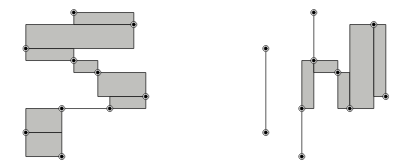
\includegraphics[width=\linewidth]{img/strips.png}
  \caption{Vertical and horizontal strips.}
  \label{fig:strips}
\end{figure}
\subsection{Algorithm to locate strips}
\begin{algorithm}[H]
\SetAlgoLined
 \caption{LocateStrip}
\KwResult{HS and VS as lists of tuples. (respectively horizontal strips and vertical strips}
 HS = \o\;
 VS = \o\;
 Calculate $O_i$ and $A_i$ $|$ $ \forall i \in [1,4]$\;
 \For{i=1 to n}{
 	\uIf{$t_i = O_3(O_1(t_i))$}{
 		$HS = HS\cup (t_i,O_1(t_i))$\;
	}
 	\uIf{$t_i = O_4(O_2(t_i))$}{
 		$HS = HS\cup (t_i,O_2(t_i))$\;
 	}
 	\uIf{$t_i = A_3(A_1(t_i))$}{
 		$VS = VS\cup (t_i,A_1(t_i))$\;
 	}
 	\uIf{$t_i = A_4(A_2(t_i))$}{
 		$VS = VS\cup (t_i,A_2(t_i))$\;
 	}
 }
 return HS and VS\;
\end{algorithm}

\section{Staircases}%%%%%%%%%%%%%%%%%%%%%%%%%%%%%%%%%%%%%%%%%%%%
Staircases are another geometric shape with a specific configuration.
\begin{figure}[H]
  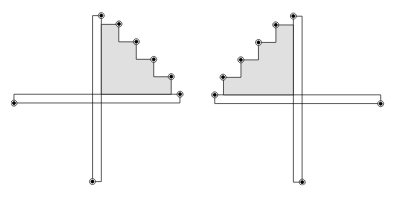
\includegraphics[width=\linewidth]{img/staircases.png}
  \caption{Staircases configuration.}
  \label{fig:staircases} 
\end{figure}

Here above on \emph{Fig 8.3} are presented two of the four possible staircases configuration.

As you can see a staircase is built on two strips, one vertical and the other one horizontal. Also note the position of the points on the strips. The points must be on a disposition where the points on the staircase side are part of the staircase itself.
\section{The resulting set}%%%%%%%%%%%%%%%%%%%%%%%%%%%%%%%%%%%
Now that we have strips and staircases we can create a generating set.

In fact all strips combined with all staircases are a generating set for our cloud of points.

Meaning that at this point we can now with the data that we have, instead of treating all terminals we can just focus on our staircases and strips.\newline

All of the done work reaches this point. What is missing for me is to properly locate staircases, and implement an approximating algorithm described [2] to calculate a minimal Manhattan network. 


\part{Conclusion and annexes}
\chapter{Internship proceeding}
This chapter is here to summarize quickly how did the internship went on, and what were the encountered difficulties.
\section{Covid-19 situation}
Due to the current situation the internship was made from my own home, as the confinement restriction didn't allowed me to work directly at the laboratory.

In this respect, the internship was for me a little harder as communicating with my internship mentors via e-mails was slower than asking direct questions to them. However they never missed on answering my questions and with a really helpful accuracy.

I hope that to a certain extent that due to this situation the internship was slowed and it was harder for me to work. I personally think that working from home is fine but not optimal, as the environment is not meant for working is would rather have worked directly at the laboratory to be more productive and efficient.

\section{Encountered difficulties}
Most of the difficulties that I encountered was the consequence of the lack of knowledge on some specific topic. I was just stuck one time in my work, while calculating the Pareto envelope of a set of points. Hopefully after a few mails to my internship's mentor, they redirected me to research papers and publication where all of what I needed was explained.

Also during visio-conferences they explained me a lot of the properties hold by Pareto envelopes, and staircases.\newline

However during the internship we had a lot of final exams and numerous other semester's projects to send to our professors. This took a lot of the work time that I could have added to this internship. A lot of work had to be done in the same as this internship and managing our time was really hard for us. I hope that in view of this situation you understand that I did my best and produced the best work I could.

\section{Current status of the work}
In terms of code, my strategy was to code by implementing tests first. This technique was tough to me last year and it proved it's effectiveness again here.

As a consequence coding all tests before implementing my own code was a big guideline for me to know where I am in my work. This internship also tough me how to organize myself in the regard of a project in order to have clear and neat code.\newline 

My aim was to reach a point where i can compute a minimal Manhattan network, which is on a good way to be done. For now i did all the work needed to recognize Pareto envelope and to get the strips and staircases set.
The last part of my work which will be done in the next three weeks is to initiate myself to linear programming (for personal knowledge), and lastly in order to compute a MMN I need to implement a 2.5 approximating algorithm that does it.\newline

I was hopping to finish all of my work before presenting you this report so that I could completely explain all of my work, but due to the current situation this was too hard to do. Hopefully my internship is giving me, I think, enough time to do the rest of my work.

\section{Continuation of the internship}
Finally i have to say that my internship is not finished and I will continue to work from home during approximately three weeks which will be enough to finish my work on this internship.

As this report is a manifest of the end of the matter "Stage ou projet - S6", I would like to thank some people before ending this work. 
\chapter{Acknowledgment}

In this last chapter i would like firstly to thank you for reading this report. I hope that this was accurate enough and that this was constructing for you. For this internship I have to thank a lot of people that helped me through this adventure.\newline

\section{Internship's mentors}
With all the work i produced, i would also like to thank Mr.Chepoi and Mr.Vaxes my intership's mentors, who despite the current covid-19 situation helped me. 

With visio-conferences and mail exchanges they managed to keep me interested in research and especially in this subject matter. I cannot count the answers that they gave to the millions of questions that i had and always with a pedagogic approach.

Even though this internship's subject was hard they always pushed me to try and understand, search, and learn what i needed to know to move forward.

In this confinement circumstances, while home working I didn't felt alone at any time. When I had questions, my internship's mentor gave me enough information so that I could work by myself. The objective of this internship was to make me learn more about research, ho it is done and of course learn more about Pareto envelopes and Manhattan networks.\newline

I personally feel that i did even more than that, I had to learn how to read scientific publications, how to search information in a bibliography, how to retrieve from Internet publish articles, understand how do some data structures works without knowing them before. 

I had to prepare small talks for my visio-conferences with Mr.Vaxes and Mr.Chepoi, to explain what did I learn, what did I do, and what were my questions. I learned a lot on paper writing also.

\section{Making this internship possible}
Preparing all of the required papers for an internship is compulsory and a long work. And I cannot end this paper without showing how much grateful I am to three particular persons.

Especially in the current sanitation situation, retrieving all the needed papers, and all needed signatures was not a soft task to do. Alone i would never have been able to do so.\newline

For this I have to gratefully thank Mme.JAMET and Mme.JEANSON whom helped me a lot with the paperwork for the University side.I took some time to understand what was wanted from me. But after starting the procedures, and mails after mails Mme.JEANSON and Mme.JAMET always answered me with astonishing rapidity and accurate instructions. And for this thank again.

For the laboratory side, I need to thank Mmme.COMES, my interlocutor for the LIS. She also help me to summaries and centralize all of my papers while starting this internship.

The current situation was not really usual but even in hard times Mme.JAMET, Mme.JEANSON and Mme.Comes helped me in making this internship possible. Nothing of this was going to be real and possible if they were not here.
\chapter{Bibliography and sources}
\underline{\textbf{Template used:}}
\begin{quoting} \begin{verbatim}
[Number] -{Autors}
         - Title of the scientific publication
         - Event/Congress where the paper was presented
{Links related to this source (Abstract and/or part of the paper as PDF)}
\end{verbatim} \end{quoting} 

\underline{\textbf{Sources:}}
\begin{quoting} \begin{verbatim}
[1] -M.Benkert, A.Wolff, F.Widmann, and T.Shirabe,
    -The minimum Manhattan network problem:approximations and exact solutions,
    -Comput.Geom.35 (2006) 188–208
pdf: https://www.sciencedirect.com/science/article/pii/S0925772105000933

[2] -N.Catusse, V.Chepoi, K.Nouioua, and Y.Vax`es,
    -Minimum Manhattan network problem in normedplanes with polygonal balls: 
     a factor 2.5 approximation algorithm,
    -Algorithmica 63 (2012) 551–567.
abstract: https://arxiv.org/abs/1004.5517
pdf:      https://arxiv.org/pdf/1004.5517.pdf

[3] -V. Chepoi, K. Nouioua, and Y. Vax`es,
    -A rounding algorithm for approximating minimum Manhat-tan networks, 
    -Theor. Comput. Sci. 390 (2008), 56–69 and APPROX-RANDOM 2005, pp. 40–51.
abstract: https://www.sciencedirect.com/science/article/pii/S0304397507007657
pdf     : Check in the link the "Download full text pdf" field.

[4] -M.Benkert, A.Wolff, F.Widmann, and T.Shirabe 
    -The minimum Manhattan network problem:approximations and exact solutions,
    -Comput.Geom.35 (2006) 188–208.
https://link.springer.com/content/pdf/10.1007/s00454-011-9342-z.pdf

[5] -A.Das, K.Fleszar, S.G.Kobourov, J.Spoerhase, S.Veeramoni, A.Wolff,
    -Approximating thegeneralized minimum Manhattan network problem,
    -Algorithmica 80 (2018), 1170-1190.
abstract: https://link.springer.com/article/10.1007/s00453-017-0298-0

[6] -A.Das, E.R.Gansner, M.Kaufmann, S.G.Kobourov, J.Spoerhase, A.Wolff,
    -Approximatingminimum Manhattan networks in higher dimensions,
    -Algorithmica 71 (2015), 36–52.
abstract: https://link.springer.com/chapter/10.1007/978-3-642-23719-5_5

[7] -J.Gudmundsson, C.Levcopoulos, and G.Narasimhan,
    -Approximating a minimum Manhattan net-work.
    -Theor.Comput.Sci.390 (2008), 56–69 and APPROX-RANDOM 2005, pp.40–51.
https://core.ac.uk/download/pdf/82701447.pdf

[8] -K.Nouioua, 
    -Pareto envelopes and Manhattan networks: Algorithmic caracterisation 
    -Computer science Thesis, University of Mediterranee, 2005.
pdf : http://pageperso.lif.univ-mrs.fr/~karim.nouioua/download/THESE_NOUIOUA.pdf
\end{verbatim} \end{quoting}





\end{document}
